% GENERATED by scripts/make_iise_manuscript.py -- do not edit by hand.
\documentclass[11pt]{article}
\usepackage[margin=1in]{geometry}
\usepackage{setspace}
\usepackage{amsmath}
\usepackage{amssymb}
\usepackage{amsthm}
\usepackage{graphicx}
\usepackage{booktabs}
\usepackage{tabularx}
\usepackage[section]{placeins}
\usepackage[authoryear,round]{natbib}
\usepackage{seqsplit}
\usepackage{url}
\usepackage{xr}
\externaldocument[S-]{supplement_iise}

\newtheorem{proposition}{Proposition}[section]
\newtheorem{theorem}{Theorem}[section]
\newtheorem{lemma}{Lemma}[section]
\newtheorem{corollary}{Corollary}[section]

% Generated by scripts/create_results_macros.py from outputs/*.json -- do not hand-edit.
\def\TracksTableRows{B --- GSM8K, homog. & 40/40 & 100.0 & 100.0 & 100.0 & -- \\
B$'$ --- GSM8K, heterog. & 40/40 & \textbf{100.0} & \textbf{100.0} & 95.0 & -- \\
C --- MATH L5, homog. & 134/134 & 89.6 & \textbf{91.0} & 89.6 & 90.3 \\
C$'$ --- MATH L5, heterog. & 134/134 & 88.1 & \textbf{90.3} & 79.1 & 79.9 \\
D --- AIME 2026, homog. & 30/30 & 80.0 & 86.7 & \textbf{90.0} & 83.3 \\
D$'$ --- AIME 2026, heterog. & 30/30 & 86.7 & \textbf{93.3} & 63.3 & 90.0 \\
E --- GPQA Diamond, homog. & 198/198 & 75.3 & \textbf{78.8} & \textbf{78.8} & 78.3 \\
E$'$ --- GPQA Diamond, heterog. & 198/198 & 74.7 & 77.3 & \textbf{79.3} & 72.7 \\
F --- AIME 2025, homog. & 30/30 & 80.0 & \textbf{83.3} & 76.7 & 86.7 \\
G --- MMLU-Pro, homog. & 100/100 & 85.0 & \textbf{86.0} & \textbf{86.0} & 83.0 \\}
\def\PairedTableRows{B --- GSM8K, homog. & 0/0 & -- & 0/0 & -- & -- & -- \\
B$'$ --- GSM8K, heterog. & 0/2 & 0.500 & 0/2 & 0.500 & -- & -- \\
C --- MATH L5, homog. & 0/2 & 0.500 & 1/1 & 1.000 & 1/2 & 1.000 \\
C$'$ --- MATH L5, heterog. & 0/15 & $<$0.001 & 4/16 & 0.012 & 7/8 & 1.000 \\
D --- AIME 2026, homog. & 1/0 & 1.000 & 3/0 & 0.250 & 2/0 & 0.500 \\
D$'$ --- AIME 2026, heterog. & 0/9 & 0.004 & 0/7 & 0.016 & 1/9 & 0.021 \\
E --- GPQA Diamond, homog. & 6/6 & 1.000 & 13/6 & 0.167 & 9/8 & 1.000 \\
E$'$ --- GPQA Diamond, heterog. & 10/6 & 0.454 & 20/11 & 0.150 & 24/11 & 0.041 \\
F --- AIME 2025, homog. & 1/3 & 0.625 & 1/2 & 1.000 & 1/4 & 0.375 \\
G --- MMLU-Pro, homog. & 2/2 & 1.000 & 3/2 & 1.000 & 5/2 & 0.453 \\}
\def\HomogPooledN{532}
\def\HomogPooledB{10}
\def\HomogPooledC{13}
\def\HomogPooledP{$p=0.678$}
\def\TotalProblems{532}
\def\FigLabels{GSM8K,GSM8K-H,MATH5,MATH5-H,AIME,AIME-H,GPQA,GPQA-H,AIME25,MMLU-Pro}
\def\FigGRCoordinates{(GSM8K,100.0) (GSM8K-H,100.0) (MATH5,89.6) (MATH5-H,88.1) (AIME,80.0) (AIME-H,86.7) (GPQA,75.3) (GPQA-H,74.7) (AIME25,80.0) (MMLU-Pro,85.0)}
\def\FigSCCoordinates{(GSM8K,100.0) (GSM8K-H,100.0) (MATH5,91.0) (MATH5-H,90.3) (AIME,86.7) (AIME-H,93.3) (GPQA,78.8) (GPQA-H,77.3) (AIME25,83.3) (MMLU-Pro,86.0)}
\def\FigORCoordinates{(GSM8K,100.0) (GSM8K-H,95.0) (MATH5,89.6) (MATH5-H,79.1) (AIME,90.0) (AIME-H,63.3) (GPQA,78.8) (GPQA-H,79.3) (AIME25,76.7) (MMLU-Pro,86.0)}
\def\FigKYCoordinates{(MATH5,90.3) (MATH5-H,79.9) (AIME,83.3) (AIME-H,90.0) (GPQA,78.3) (GPQA-H,72.7) (AIME25,86.7) (MMLU-Pro,83.0)}
\def\HeteroPooledN{402}
\def\HeteroPooledB{10}
\def\HeteroPooledC{32}
\def\HeteroPooledP{$p<0.001$}
\def\ExtendedTableRows{C --- MATH L5, homog. & 132 & 90.9 & 92.4 & 2 & 89.6 & 91.0 \\
C$'$ --- MATH L5, heterog. & 131 & 79.4 & 90.8 & 3 & 79.1 & 90.3 \\
D --- AIME 2026, homog. & 24 & 95.8 & 91.7 & 6 & 90.0 & 86.7 \\
D$'$ --- AIME 2026, heterog. & 23 & 78.3 & 100.0 & 7 & 63.3 & 93.3 \\
E --- GPQA Diamond, homog. & 175 & 82.3 & 82.9 & 23 & 78.8 & 78.8 \\
E$'$ --- GPQA Diamond, heterog. & 163 & 85.3 & 82.8 & 35 & 79.3 & 77.3 \\
F --- AIME 2025, homog. & 24 & 87.5 & 95.8 & 6 & 76.7 & 83.3 \\
G --- MMLU-Pro, homog. & 94 & 88.3 & 88.3 & 6 & 86.0 & 86.0 \\}
\def\CoverageTableRows{B --- GSM8K, homog. & 40 & 40 & 0 & 0 & 0 & -- \\
B$'$ --- GSM8K, heterog. & 40 & 40 & 0 & 0 & 0 & 40 \\
C --- MATH L5, homog. & 134 & 134 & 0 & 0 & 0 & -- \\
C$'$ --- MATH L5, heterog. & 134 & 134 & 0 & 0 & 0 & 131 \\
D --- AIME 2026, homog. & 30 & 30 & 0 & 0 & 0 & -- \\
D$'$ --- AIME 2026, heterog. & 30 & 30 & 0 & 0 & 0 & 23 \\
E --- GPQA Diamond, homog. & 198 & 198 & 0 & 0 & 0 & -- \\
E$'$ --- GPQA Diamond, heterog. & 198 & 198 & 0 & 0 & 0 & 80 \\
F --- AIME 2025, homog. & 30 & 30 & 0 & 0 & 0 & -- \\
G --- MMLU-Pro, homog. & 100 & 100 & 0 & 0 & 0 & -- \\}
\def\KYTopOneN{854}
\def\KYTopOneDiffers{139}
\def\KYORwins{50}
\def\KYKYwins{44}
\def\NGSMh{40}
\def\TotGSMh{40}
\def\AccORGSMh{100.0}
\def\AccSCGSMh{100.0}
\def\AccGRGSMh{100.0}
\def\DiscGSMh{0}
\def\ORwinsGSMh{0}
\def\SCwinsGSMh{0}
\def\LegacyGSMh{0}
\def\NGSMx{40}
\def\TotGSMx{40}
\def\AccORGSMx{95.0}
\def\AccSCGSMx{100.0}
\def\AccGRGSMx{100.0}
\def\DiscGSMx{2}
\def\ORwinsGSMx{0}
\def\SCwinsGSMx{2}
\def\LegacyGSMx{40}
\def\NMATHh{134}
\def\TotMATHh{134}
\def\AccORMATHh{89.6}
\def\AccSCMATHh{91.0}
\def\AccGRMATHh{89.6}
\def\AccKYMATHh{90.3}
\def\DiscMATHh{2}
\def\ORwinsMATHh{0}
\def\SCwinsMATHh{2}
\def\LegacyMATHh{0}
\def\NMATHx{134}
\def\TotMATHx{134}
\def\AccORMATHx{79.1}
\def\AccSCMATHx{90.3}
\def\AccGRMATHx{88.1}
\def\AccKYMATHx{79.9}
\def\DiscMATHx{15}
\def\ORwinsMATHx{0}
\def\SCwinsMATHx{15}
\def\LegacyMATHx{131}
\def\NAIMEh{30}
\def\TotAIMEh{30}
\def\AccORAIMEh{90.0}
\def\AccSCAIMEh{86.7}
\def\AccGRAIMEh{80.0}
\def\AccKYAIMEh{83.3}
\def\DiscAIMEh{1}
\def\ORwinsAIMEh{1}
\def\SCwinsAIMEh{0}
\def\LegacyAIMEh{0}
\def\NAIMEx{30}
\def\TotAIMEx{30}
\def\AccORAIMEx{63.3}
\def\AccSCAIMEx{93.3}
\def\AccGRAIMEx{86.7}
\def\AccKYAIMEx{90.0}
\def\DiscAIMEx{9}
\def\ORwinsAIMEx{0}
\def\SCwinsAIMEx{9}
\def\LegacyAIMEx{23}
\def\NGPQAh{198}
\def\TotGPQAh{198}
\def\AccORGPQAh{78.8}
\def\AccSCGPQAh{78.8}
\def\AccGRGPQAh{75.3}
\def\AccKYGPQAh{78.3}
\def\DiscGPQAh{12}
\def\ORwinsGPQAh{6}
\def\SCwinsGPQAh{6}
\def\LegacyGPQAh{0}
\def\NGPQAx{198}
\def\TotGPQAx{198}
\def\AccORGPQAx{79.3}
\def\AccSCGPQAx{77.3}
\def\AccGRGPQAx{74.7}
\def\AccKYGPQAx{72.7}
\def\DiscGPQAx{16}
\def\ORwinsGPQAx{10}
\def\SCwinsGPQAx{6}
\def\LegacyGPQAx{80}
\def\NAIME25h{30}
\def\TotAIME25h{30}
\def\AccORAIME25h{76.7}
\def\AccSCAIME25h{83.3}
\def\AccGRAIME25h{80.0}
\def\AccKYAIME25h{86.7}
\def\DiscAIME25h{4}
\def\ORwinsAIME25h{1}
\def\SCwinsAIME25h{3}
\def\LegacyAIME25h{0}
\def\NMMLUh{100}
\def\TotMMLUh{100}
\def\AccORMMLUh{86.0}
\def\AccSCMMLUh{86.0}
\def\AccGRMMLUh{85.0}
\def\AccKYMMLUh{83.0}
\def\DiscMMLUh{4}
\def\ORwinsMMLUh{2}
\def\SCwinsMMLUh{2}
\def\LegacyMMLUh{0}
\def\RBOverallAcc{60.5}
\def\RBN{161}
\def\RBCILow{53.2}
\def\RBCIHigh{68.1}
\def\RBChatAcc{68.6}
\def\RBChatRows{35}
\def\RBChatCorrect{24}
\def\RBReasoningAcc{73.5}
\def\RBReasoningRows{49}
\def\RBReasoningCorrect{36}
\def\RBChatHardAcc{42.9}
\def\RBChatHardRows{42}
\def\RBChatHardCorrect{18}
\def\RBSafetyAcc{57.1}
\def\RBSafetyRows{35}
\def\RBSafetyCorrect{20}
\def\RBMicroAcc{60.9}
\def\RBXOverallAcc{48.5}
\def\RBXN{161}
\def\RBXCILow{40.9}
\def\RBXCIHigh{56.1}
\def\RBXChatAcc{65.7}
\def\RBXChatRows{35}
\def\RBXChatCorrect{23}
\def\RBXReasoningAcc{57.1}
\def\RBXReasoningRows{49}
\def\RBXReasoningCorrect{28}
\def\RBXChatHardAcc{31.0}
\def\RBXChatHardRows{42}
\def\RBXChatHardCorrect{13}
\def\RBXSafetyAcc{40.0}
\def\RBXSafetyRows{35}
\def\RBXSafetyCorrect{14}
\def\RBXMicroAcc{48.4}
\def\RBChosenLongerK{54}
\def\RBChosenLongerN{79}
\def\RBChosenLongerAcc{68.4}
\def\RBChosenLongerCILow{57.5}
\def\RBChosenLongerCIHigh{77.6}
\def\RBRejectedLongerK{44}
\def\RBRejectedLongerN{82}
\def\RBRejectedLongerAcc{53.7}
\def\RBRejectedLongerCILow{42.9}
\def\RBRejectedLongerCIHigh{64.0}

% Generated by scripts/analyze_selection.py from outputs/*.json -- do not hand-edit.
\def\FloorGSMh{99.2}
\def\OracleGSMh{100.0}
\def\FloorGSMx{97.5}
\def\OracleGSMx{100.0}
\def\FloorMATHh{89.8}
\def\OracleMATHh{91.8}
\def\FloorMATHx{82.6}
\def\OracleMATHx{92.4}
\def\FloorAIMEh{85.6}
\def\OracleAIMEh{90.0}
\def\FloorAIMEx{78.7}
\def\OracleAIMEx{96.0}
\def\FloorGPQAh{77.3}
\def\OracleGPQAh{87.7}
\def\FloorGPQAx{76.3}
\def\OracleGPQAx{92.2}
\def\RecoveryTableRows{B --- GSM8K, homog. & 40 & 99.2 & 100.0 & 100.0 & 100.0 & 100 & 100 \\
B$'$ --- GSM8K, heterog. & 40 & 97.5 & 100.0 & 95.0 & 100.0 & 100 & -100 \\
C --- MATH L5, homog. & 134 & 89.8 & 91.0 & 89.6 & 91.8 & 62 & -12 \\
C$'$ --- MATH L5, heterog. & 131 & 82.6 & 90.8 & 79.4 & 92.4 & 84 & -32 \\
D --- AIME 2026, homog. & 30 & 85.6 & 86.7 & 90.0 & 90.0 & 25 & 100 \\
D$'$ --- AIME 2026, heterog. & 25 & 78.7 & 96.0 & 72.0 & 96.0 & 100 & -38 \\
E --- GPQA Diamond, homog. & 195 & 77.3 & 79.0 & 79.0 & 87.7 & 16 & 16 \\
E$'$ --- GPQA Diamond, heterog. & 90 & 76.3 & 83.3 & 83.3 & 92.2 & 44 & 44 \\}
\def\SelectionTableRows{Nemotron-3.5 (judge model) & 572 & 87.6 & 19 (7.9\%) & 100.0 \\
North-Mini-Code & 572 & 87.2 & 168 (69.7\%) & 81.5 \\
Laguna-S 2.1 & 546 & 73.3 & 53 (22.0\%) & 67.9 \\
Xing4.0-29B & 26 & 50.0 & 1 (0.4\%) & 0.0 \\}
\def\SelectionRows{286}
\def\PickShareNemotron{7.9}
\def\CandAccNemotron{87.6}
\def\PickAccNemotron{100.0}
\def\CandNNemotron{572}
\def\PickShareCohere{69.7}
\def\CandAccCohere{87.2}
\def\PickAccCohere{81.5}
\def\CandNCohere{572}
\def\PickShareLaguna{22.0}
\def\CandAccLaguna{73.3}
\def\PickAccLaguna{67.9}
\def\CandNLaguna{546}
\def\PickShareXingchen{0.4}
\def\CandAccXingchen{50.0}
\def\PickAccXingchen{0.0}
\def\CandNXingchen{26}
\def\SelectionTopSharePct{69.7}
\def\SelectionXingchenCands{26}
\def\LongestPickHomK{18}
\def\LongestPickHomN{359}
\def\LongestPickHomChance{33}
\def\LongestPickHomPct{5}
\def\WinnerLenRatioHom{0.67}
\def\LongestPickHetK{2}
\def\LongestPickHetN{246}
\def\LongestPickHetChance{17}
\def\LongestPickHetPct{1}
\def\WinnerLenRatioHet{0.45}

% Generated by scripts/ablation_weights_offline.py from outputs/*.json -- do not hand-edit.
\def\AblationTableRows{B$'$ GSM8K, heterog. & 38/40 & 100.0 & 94.7 & 100.0 & 100.0 & 100.0 \\
C MATH L5, homog. & 25/134 & 84.0 & 84.0 & 84.0 & 84.0 & 84.0 \\
C$'$ MATH L5, heterog. & 133/134 & 90.2 & 78.9 & 82.7 & 82.7 & 87.2 \\
D AIME 2026, homog. & 9/30 & 66.7 & 66.7 & 66.7 & 66.7 & 66.7 \\
D$'$ AIME 2026, heterog. & 29/30 & 93.1 & 62.1 & 75.9 & 75.9 & 96.6 \\
E GPQA Diamond, homog. & 168/198 & 77.4 & 78.0 & 78.0 & 78.0 & 76.2 \\
E$'$ GPQA Diamond, heterog. & 197/198 & 77.2 & 79.2 & 72.1 & 71.1 & 75.6 \\
F AIME 2025, homog. & 30/30 & 83.3 & 76.7 & 83.3 & 83.3 & 83.3 \\
G MMLU-Pro, homog. & 100/100 & 86.0 & 86.0 & 84.0 & 84.0 & 86.0 \\}
\def\AblationFidelityK{729}
\def\AblationFidelityN{729}
\def\AblHomN{332}
\def\AblHomDefAcc{80.4}
\def\AblHomDefB{9}
\def\AblHomDefC{10}
\def\AblHomDefP{1.000}
\def\AblHomNoCostAcc{80.4}
\def\AblHomNoCostB{11}
\def\AblHomNoCostC{12}
\def\AblHomNoCostP{1.000}
\def\AblHomQOnlyAcc{80.4}
\def\AblHomQOnlyB{11}
\def\AblHomQOnlyC{12}
\def\AblHomQOnlyP{1.000}
\def\AblHomSCQAcc{80.1}
\def\AblHomSCQB{2}
\def\AblHomSCQC{4}
\def\AblHomSCQP{0.688}
\def\AblHomSCAcc{80.7}
\def\AblHetN{397}
\def\AblHetDefAcc{79.3}
\def\AblHetDefB{10}
\def\AblHetDefC{32}
\def\AblHetDefP{$<$0.001}
\def\AblHetNoCostAcc{78.6}
\def\AblHetNoCostB{9}
\def\AblHetNoCostC{34}
\def\AblHetNoCostP{$<$0.001}
\def\AblHetQOnlyAcc{78.1}
\def\AblHetQOnlyB{9}
\def\AblHetQOnlyC{36}
\def\AblHetQOnlyP{$<$0.001}
\def\AblHetSCQAcc{83.4}
\def\AblHetSCQB{1}
\def\AblHetSCQC{7}
\def\AblHetSCQP{0.070}
\def\AblHetSCAcc{84.9}
\def\CostSpreadMed{0.88}
\def\QualitySpreadMed{0.20}
\def\CostDominatesK{653}
\def\CostDominatesN{729}

% Generated by scripts/baselines_extra_offline.py from outputs/*.json -- do not hand-edit.
\def\BaseHomshortestAcc{84.6}
\def\BaseHomshortestN{532}
\def\BaseHomshortestB{10}
\def\BaseHomshortestC{15}
\def\BaseHetshortestAcc{78.4}
\def\BaseHetshortestN{402}
\def\BaseHetshortestB{11}
\def\BaseHetshortestC{38}
\def\BaseHomlongestAcc{83.3}
\def\BaseHomlongestN{532}
\def\BaseHomlongestB{11}
\def\BaseHomlongestC{23}
\def\BaseHetlongestAcc{80.1}
\def\BaseHetlongestN{402}
\def\BaseHetlongestB{5}
\def\BaseHetlongestC{25}
\def\BaseHommbrAcc{85.9}
\def\BaseHommbrN{532}
\def\BaseHommbrB{9}
\def\BaseHommbrC{7}
\def\BaseHetmbrAcc{85.3}
\def\BaseHetmbrN{402}
\def\BaseHetmbrB{9}
\def\BaseHetmbrC{8}
\def\BaseHomconfargmaxAcc{80.7}
\def\BaseHomconfargmaxN{332}
\def\BaseHomconfargmaxB{7}
\def\BaseHomconfargmaxC{7}
\def\BaseHetconfargmaxAcc{79.8}
\def\BaseHetconfargmaxN{397}
\def\BaseHetconfargmaxB{10}
\def\BaseHetconfargmaxC{30}
\def\BaseHomconfvoteAcc{79.8}
\def\BaseHomconfvoteN{332}
\def\BaseHomconfvoteB{0}
\def\BaseHomconfvoteC{3}
\def\BaseHetconfvoteAcc{84.4}
\def\BaseHetconfvoteN{397}
\def\BaseHetconfvoteB{3}
\def\BaseHetconfvoteC{5}
\def\BaseHomtournamentAcc{79.8}
\def\BaseHomtournamentN{332}
\def\BaseHomtournamentB{11}
\def\BaseHomtournamentC{14}
\def\BaseHettournamentAcc{79.6}
\def\BaseHettournamentN{397}
\def\BaseHettournamentB{12}
\def\BaseHettournamentC{33}
\def\BaseHombtAcc{80.1}
\def\BaseHombtN{332}
\def\BaseHombtB{10}
\def\BaseHombtC{12}
\def\BaseHetbtAcc{77.8}
\def\BaseHetbtN{397}
\def\BaseHetbtB{8}
\def\BaseHetbtC{36}
\def\BaselineTableRows{Shortest candidate & 532 & 84.6 (85.5) & 10/15 & 0.424 & 402 & 78.4 (85.1) & 11/38 & $<$0.001 \\
Longest candidate & 532 & 83.3 (85.5) & 11/23 & 0.058 & 402 & 80.1 (85.1) & 5/25 & $<$0.001 \\
MBR (Jaccard) & 532 & 85.9 (85.5) & 9/7 & 0.804 & 402 & 85.3 (85.1) & 9/8 & 1.000 \\
Confidence argmax$^\dagger$ & 332 & 80.7 (80.7) & 7/7 & 1.000 & 397 & 79.8 (84.9) & 10/30 & 0.002 \\
Confidence-weighted vote$^\dagger$ & 332 & 79.8 (80.7) & 0/3 & 0.250 & 397 & 84.4 (84.9) & 3/5 & 0.727 \\
Knockout tournament$^\dagger$ & 332 & 79.8 (80.7) & 11/14 & 0.690 & 397 & 79.6 (84.9) & 12/33 & 0.002 \\
Bradley--Terry$^\dagger$ & 332 & 80.1 (80.7) & 10/12 & 0.832 & 397 & 77.8 (84.9) & 8/36 & $<$0.001 \\}

% Generated by scripts/judge_threshold_theory.py -- do not hand-edit.
\def\ThresholdRows{0.2 & 0.565 \\
0.4 & 0.631 \\
0.5 & 0.667 \\
0.6 & 0.706 \\
0.7 & 0.750 \\
0.8 & 0.804 \\
0.9 & 0.875 \\}
\def\ThresholdEmpiricalRows{GPQA Diamond & 0.773 & 72 & 0.536 & 0.788 \\}
\def\ThresholdHeteroRows{GSM8K & 0.975 & 24 & 0.660 \\
MATH L5 & 0.826 & 283 & 0.532 \\
AIME 2026 & 0.787 & 112 & 0.552 \\
GPQA Diamond & 0.763 & 234 & 0.477 \\}

% Generated by scripts/judge_threshold_general.py -- do not hand-edit.
\def\ThresholdNRows{3 & 0.667 & 0.804 & 0.625 & 0.782 \\
4 & 0.759 & 0.891 & 0.675 & 0.814 \\
5 & 0.800 & 0.919 & 0.682 & 0.824 \\
6 & 0.825 & 0.935 & 0.679 & 0.819 \\}
\def\ThresholdValidationRows{4 & 0.5 & 0.0 & 0.7 & -5.40 & -5.50 $\pm$ 0.11 \\
5 & 0.8 & 0.5 & 0.8 & -0.66 & -0.68 $\pm$ 0.05 \\
6 & 0.5 & 0.5 & 0.7 & +2.64 & +2.65 $\pm$ 0.11 \\
6 & 0.8 & 0.0 & 0.9 & -0.20 & -0.20 $\pm$ 0.01 \\}
\def\PairDepInside{30}\def\PairDepTrials{30}

% Generated by scripts/judge_threshold_empirical.py -- do not hand-edit.
\def\ThresholdEmpGenRows{GPQA Diamond & 3 & 0.773 & 0.88 & 0.536 & 0.788 & 0.716 \\
GSM8K-H & 6 & 0.975 & 1.00 & 0.660 & 0.995 & 0.904 \\
MATH L5-H & 6 & 0.826 & 0.69 & 0.532 & 0.944 & 0.787 \\
AIME 2026-H & 6 & 0.787 & 0.20 & 0.552 & 0.930 & 0.894 \\
GPQA Diamond-H & 6 & 0.763 & 0.85 & 0.477 & 0.921 & 0.703 \\}

% Generated by scripts/judge_threshold_extensions.py -- do not hand-edit.
\def\ThresholdNSevenRow{7 & 0.841 & 0.945 & 0.673 & 0.821 \\}
\def\ThresholdDRows{1 & 0.500 & 0.669 & 0.500 & 0.721 \\
2 & 0.594 & 0.754 & 0.592 & 0.770 \\
3 & 0.640 & 0.791 & 0.638 & 0.798 \\
8 & 0.710 & 0.847 & 0.723 & 0.854 \\
$\infty$ & 0.759 & 0.891 & 0.800 & 0.919 \\}
\def\ThresholdLambdaRows{0.5 & 0.693 & 0.820 & 0.825 \\
0.6 & 0.916 & 0.867 & 0.862 \\
0.7 & 1.204 & 0.907 & 0.899 \\
0.8 & 1.609 & 0.943 & 0.935 \\
0.9 & 2.303 & 0.973 & 0.970 \\}
\def\ThresholdCostRows{0 & 84.5 & 96.1 \\
0.25 & 84.4 & 96.1 \\
1 & 83.9 & 94.9 \\
4 & 81.4 & 86.0 \\
$\infty$ (shortest) & 79.8 & 79.8 \\}

% Generated by scripts/create_manuscript_tables.py from outputs/runs/summarize-the-plot-of-hamlet-in-one-sentence/selection.json -- do not hand-edit.
\def\WorkedExampleTableRows{c0 & 0.606 & 1.00 & 0.20 & 38 & 0.486 \\
c1 & 0.387 & 1.00 & 0.20 & 32 & 0.327 \\
c2$^\ast$ & 0.644 & 1.00 & 0.20 & 33 & 0.574 \\
c3 & 0.575 & 1.00 & 0.20 & 38 & 0.455 \\
c4 & 0.288 & 1.00 & 0.20 & 33 & 0.218 \\}
\def\WorkedExampleWinner{c2}
\def\WorkedExampleQualityBars{(c0,0.6062) (c1,0.3875) (c2,0.6438) (c3,0.5750) (c4,0.2875)}
\def\WorkedExampleConfidenceBars{(c0,0.2000) (c1,0.2000) (c2,0.2000) (c3,0.2000) (c4,0.2000)}
\def\WorkedExampleConsistencyBars{(c0,0.0600) (c1,0.0600) (c2,0.0600) (c3,0.0600) (c4,0.0600)}
\def\WorkedExampleCostBars{(c0,-0.3800) (c1,-0.3200) (c2,-0.3300) (c3,-0.3800) (c4,-0.3300)}

% Generated by scripts/difficulty_mixture.py -- do not hand-edit.
\def\MixtureThresholdRows{0.4 & 0.654 & 0.649 & 0.641 & 0.634 & 0.631 \\
0.6 & 0.679 & 0.686 & 0.694 & 0.702 & 0.706 \\
0.8 & 0.706 & 0.727 & 0.757 & 0.788 & 0.804 \\}
\def\MixtureEmpiricalRows{AIME 2025 & 30 & 81.1 & 78.6 & 88.9 & 88.0 & 92.7 & +6.7 & +3.5 & -0.9 \\
MMLU-Pro & 100 & 85.0 & 39.3 & 82.7 & 83.5 & 80.7 & -3.7 & -3.8 & -15.1 \\
Pooled & 130 & 84.1 & 52.4 & 84.1 & 84.5 & 85.0 & -1.3 & -2.2 & -10.3 \\}
\def\MixPooledN{130}
\def\MixPooledQ{52.4}
\def\MixPooledObsCop{84.1}
\def\MixPooledPredCop{84.5}
\def\MixPooledNaiveCop{85.0}
\def\MixPooledErrLo{-1.7}
\def\MixPooledErrHi{+0.8}
\def\MixPooledGapObs{-1.3}
\def\MixPooledGapPred{-2.2}
\def\MixPooledGapNaive{-10.3}
\def\MixPooledObsVote{85.4}
\def\MixPooledPredVote{86.7}
\def\MixPooledNaiveVote{95.3}

% Generated by scripts/hybrid_rule.py -- do not hand-edit.
\def\HybridTheoryRows{3 & 0.30 & 0.6 & 36.3 & 36.5 & 41.0 \\
3 & 0.30 & 0.8 & 36.3 & 50.4 & 52.2 \\
3 & 0.60 & 0.6 & 74.4 & 67.1 & 77.5 \\
3 & 0.60 & 0.8 & 74.4 & 80.7 & 84.8 \\
3 & 0.85 & 0.6 & 95.8 & 88.6 & 96.4 \\
3 & 0.85 & 0.8 & 95.8 & 94.9 & 97.9 \\
6 & 0.30 & 0.6 & 63.0 & 43.6 & 66.7 \\
6 & 0.30 & 0.8 & 63.0 & 70.7 & 77.1 \\
6 & 0.60 & 0.6 & 96.5 & 73.9 & 97.0 \\
6 & 0.60 & 0.8 & 96.5 & 93.3 & 98.2 \\
6 & 0.85 & 0.6 & 100.0 & 91.7 & 100.0 \\
6 & 0.85 & 0.8 & 100.0 & 98.8 & 100.0 \\}
\def\HybHomN{164}
\def\HybHomTies{11}
\def\HybHomOpp{6}
\def\HybHomSC{84.1}
\def\HybHomCop{83.5}
\def\HybHomHyb{84.1}
\def\HybHomBSC{1}
\def\HybHomCSC{1}
\def\HybHomBCop{4}
\def\HybHomCCop{3}
\def\HybHomPSC{1.000}
\def\HybHomPCop{1.000}
\def\HybHetN{200}
\def\HybHetTies{11}
\def\HybHetOpp{8}
\def\HybHetSC{92.5}
\def\HybHetCop{85.5}
\def\HybHetHyb{92.0}
\def\HybHetBSC{1}
\def\HybHetCSC{2}
\def\HybHetBCop{14}
\def\HybHetCCop{1}
\def\HybHetPSC{1.000}
\def\HybHetPCop{$<$0.001}
\def\HybridAuditRows{Hom. AIME 2025 & 30 & 4/2 & 83.3 & 90.0 & 83.3 & 1/1 (1.000) & 0/2 (0.500) \\
Hom. AIME 2026 & 9 & 1/0 & 66.7 & 66.7 & 66.7 & 0/0 (--) & 0/0 (--) \\
Hom. MATH L5 & 25 & 1/0 & 84.0 & 84.0 & 84.0 & 0/0 (--) & 0/0 (--) \\
Hom. MMLU-Pro & 100 & 5/4 & 86.0 & 83.0 & 86.0 & 0/0 (--) & 4/1 (0.375) \\
Hom. All & 164 & 11/6 & 84.1 & 83.5 & 84.1 & 1/1 (1.000) & 4/3 (1.000) \\
Het. AIME 2026 & 29 & 1/1 & 93.1 & 82.8 & 96.6 & 1/0 (1.000) & 4/0 (0.125) \\
Het. GSM8K & 38 & 1/1 & 100.0 & 100.0 & 100.0 & 0/0 (--) & 0/0 (--) \\
Het. MATH L5 & 133 & 9/6 & 90.2 & 82.0 & 88.7 & 0/2 (0.500) & 10/1 (0.012) \\
Het. All & 200 & 11/8 & 92.5 & 85.5 & 92.0 & 1/2 (1.000) & 14/1 ($<$0.001) \\}



\begin{document}
\setstretch{1.5}

\begin{center}
{\large\bfseries Vote First, Judge on Ties: Cost-Aware Answer Selection for Language-Model Systems}
\end{center}

\begin{abstract}
Intelligent systems built on language models often sample several answers and must return one. Designers can take the most frequent answer (self-consistency voting) at no extra cost, or pay for a pairwise judge that is itself unreliable, and they lack guidelines for choosing. We analyze the choice in a finite-pool model and audit it on stored runs. Voting first and consulting the judge only on tied answers is Bayes-optimal in the model and never worse than either voting or judging everywhere, so it needs no judge-accuracy threshold. Judging everywhere pays only above an explicit break-even accuracy (80.35\% at 80\% candidate accuracy for three candidates); when problems differ in difficulty, that break-even depends on an effective-odds ratio of difficulty moments, not on pooled accuracy. We audit one free-tier judge, scoring \RBOverallAcc\% on RewardBench, on six benchmarks of \TotalProblems{} problems. Paired exact tests find no homogeneous-pool advantage over self-consistency (\HomogPooledB{} versus \HomogPooledC{} discordant problems of \HomogPooledN{}), and judging everywhere performs worse in heterogeneous pools (\HeteroPooledB{} versus \HeteroPooledC{} of \HeteroPooledN{}, \HeteroPooledP). Vote-first selection removes that loss (\HybHetBCop{} versus \HybHetCCop{} discordant problems) with only \HybHetCallShare\% of the judge comparisons, but adds no detectable accuracy over voting because exact ties are rare. We close with design guidelines for system builders. The findings concern the tested judge, not stronger judges.
\end{abstract}

\noindent\textbf{Keywords:} Language models ; Answer selection ; Self-consistency ; LLM-as-a-judge ; Decision-level fusion ; Cost-aware design

\section{Introduction}

Intelligent systems built on language models, such as question-answering
assistants and decision-support tools, rarely return the first answer they
generate. A common design samples several candidate answers and selects one.
Two selectors are widely used. Self-consistency \citep{wang2023selfconsistency}
returns the most frequent extracted final answer at no extra cost; when all
answers differ, its result depends on the tie rule. A language-model judge can
distinguish such answers, but it is a paid component that is itself unstable
and inaccurate \citep{atil2024nondeterminism,landesberg2026bestofn}.
System designers therefore face a concrete management question: when is a
judge worth its price, and where in the pipeline should it be called? Practical
guidance is scarce, because published comparisons rarely hold the candidate
pool fixed or separate agreement with judge preferences from correctness
against ground truth. We study selection over fixed candidate pools to give
that guidance.

The operational decision arises after generation has already incurred its
cost: a system must return one of the available responses. A correct answer
may be present even when the most frequent answer is wrong, while a larger
pool may add only repeated errors. Conversely, when several independent
draws agree on the correct answer, replacing their vote with a noisy judge
can discard useful evidence. The relevant comparison is therefore between
selection rules on the same candidates, rather than between separately
generated responses. Checkable mathematics, science and knowledge questions
provide ground truth for making that comparison.

Two distinct optimization questions follow. The first is which ordering
best represents the judge's pairwise preferences. The second is which
selected answer is correct. An exact ranking solution answers the first
question but need not answer the second. OR-Select makes the selection
objective explicit, while a Kemeny--Young solution supplies a ranking
reference. The probabilistic analysis then asks a separate question: under
a specified model of correct and incorrect answers, how accurate must
binary comparisons be for their Copeland winner to outperform voting?

The paper makes five contributions. First, it proves that voting first and
judging only on ties is Bayes-optimal in a finite-pool model and weakly
dominates both plurality and judging everywhere, and it measures the judge
comparisons this saves on stored runs (Sections~\ref{sec:hybrid} and
\ref{sec:hybrid-results}). Second, it derives the exact condition under which
binary pairwise judging with Copeland aggregation beats plurality voting: a
closed form for $N=3$, enumeration for $N\le7$, and extensions to
pair-dependent judges and colliding wrong answers (Section~\ref{sec:theory} and
Online Supplement). Third, it shows that when problems differ in difficulty this
threshold is governed by an effective-odds ratio of difficulty moments, not by
pooled accuracy, and tests the per-problem prediction on stored judgments
(Sections~\ref{sec:mixture} and \ref{sec:mixture-results}). Fourth, it audits
one free-tier judge on six ground-truth benchmarks using paired tests, recovery
relative to available headroom and weight ablations
(Sections~\ref{sec:experiments}--\ref{sec:results}). Fifth, it supplies a composite
selector, OR-Select, with an exact Kemeny--Young reference and stored judge
outputs for offline comparison (Section~\ref{sec:formal-model}), and distills the
results into design guidelines (Section~\ref{sec:guidelines}).

Operationally, vote-first selection has the structure of redundant inspection
with adjudication on disagreement: several inexpensive assessments are combined
by majority, and a costlier arbiter is consulted only when they fail to agree.
Here each judge call has a price, so the question of when an additional
comparison is worth buying is a measurement-allocation decision under costly
information, and Theorem~\ref{thm:hybrid} states when this structure is optimal.

\paragraph{Outcome and use case}
\label{sec:outcome}
The tested selector has no detected advantage over voting with homogeneous
generation and performs worse in the pooled heterogeneous condition.
This does not establish that stronger judges cannot help. The threshold
analysis quantifies the reliability needed by a specified \emph{binary}
selector under its assumptions; it is not a universal deployment test for
soft-score or composite selectors. For applications with checkable answers,
the practical contribution is an audit: retain candidates and judge outputs,
compare selectors on the same problems, and distinguish ranking fit from
answer accuracy before replacing voting.

An application need not adopt the particular default weights to use this
protocol. It can store one candidate pool per problem, freeze the judge
outputs, and compare alternative aggregation or cost policies without
confounding them with new generations. Applications with a reliable final
answer extractor can include plurality directly; open-ended applications
need a separately justified grouping or evaluation rule. The distinction
between these settings matters: exact textual disagreement is not itself
evidence that responses differ in meaning or quality.

\section{Related Work}
\label{sec:related}

\paragraph{Answer selection and judges}
Universal self-consistency \citep{chen2023usc}, PAIRS \citep{liu2024pairs}
and LLM-Blender \citep{jiang2023llmblender} replace or supplement voting
with model evaluations. Verifier-based selection uses trained reward models
\citep{cobbe2021gsm8k,lightman2023letsverify}; our selector is training-free.
Preference-graph ensembling and denoising also have recovery guarantees
and response-selection applications \citep{hu2024pged}; graph aggregation
itself is therefore established prior work.
Positional bias affects judges \citep{zheng2023judging,wang2023notfair},
as does self-preference \citep{panickssery2024selfpref}.
We average input orders \citep{tang2024permutation}. Errors can be shared
\citep{kim2025correlated}; benchmark judge scores need
not predict within-prompt selection quality \citep{landesberg2026bestofn}.
Judges have also been benchmarked as test-time-scaling selectors
\citep{zhou2025jetts}, repeated pairwise judgments have been aggregated
with calibrated vote distributions \citep{dadkhahi2025calibrated}, and
knockout-style pairwise selection with repeated comparisons has been given
provable scaling laws \citep{chen2025provable}. Our setting differs in
analyzing complete finite tournaments against plurality voting and in
auditing the resulting selectors against ground truth.

Two peer-reviewed studies frame our design. Best-of-$N$ selection
against an imperfect proxy is vulnerable to reward hacking, and regularized
and stochastic variants have been compared on alignment benchmarks
\citep{ichihara2025bon}; our judge is such a proxy, which is why we score the
selected answer against ground truth instead of against the judge. A
systematic comparison of nine debiasing strategies for pairwise judges finds
style bias far larger than position bias in its benchmarks
\citep{soumik2026judging}; our order-averaging controls only position, so
style effects remain untested here (Section~\ref{sec:future}).
These findings motivate paired correctness evaluation.

These approaches also make different uses of additional information.
Universal self-consistency asks a model to identify agreement between
free-form responses; pairwise ranking evaluates relations between
responses; a trained verifier estimates correctness from task-specific
supervision. They are not interchangeable baselines. Our experiments
compare a training-free judge and stored-output selectors, and do not
estimate the performance of a separately trained verifier. The
coverage-versus-selection distinction in inference-time scaling
\citep{snell2024scaling} motivates reporting both the
availability of a correct answer and the fraction of that opportunity
actually recovered.

\paragraph{Ranking and voting}
The Kemeny--Young rule \citep{kemeny1959mathematics,young1978kemeny}
is NP-hard \citep{bartholdi1989voting}; weighted-win ranking has a known
5-approximation for disagreement \citep{coppersmith2006ordering}.
Its likelihood interpretation under a noisy ordering model
\citep{young1988condorcet,caragiannis2016noisy} is related to, but different from, our
two-class correctness model with fair same-class comparisons.
Recent analyses study reward-based selection against voting
\citep{di2025bom,komiyama2025bestofinf} and heterogeneous, correlated
ensembles \citep{ai2025beyondmv}. In particular,
\citet{komiyama2025bestofinf} report voting outperforming judges.
Our analysis instead fixes a binary pairwise rule and derives its exact
finite-pool accuracy difference from plurality. This identifies the
comparison reliability needed at a given candidate accuracy, rather than
inferring selection quality from a ranking objective alone.

The distinction from the closest inference-scaling analyses is specific.
\citet{di2025bom} combine answer frequencies and reward information in a
minimax analysis of pass-at-budget selection. \citet{komiyama2025bestofinf}
study asymptotic ensemble performance and optimized model weights, and
also compare practical selectors. \citet{ai2025beyondmv} use higher-order
information for aggregation of heterogeneous, correlated predictions.
Here the object is the finite tournament induced by binary comparisons:
the three-candidate calculation is explicit, larger small pools are
enumerated, and the empirical audit keeps candidate generation fixed
when comparing decision rules.
\citet{he2026minority} instead learn when to overturn a majority in
three-agent debates, and also report a judge losing to voting. Their
selective-intervention criterion concerns the precision of majority
overrides, rather than the mixed-pair accuracy needed by a complete
Copeland tournament. Negative judge results alone are not the distinction.

\paragraph{Decision fusion and ensembles}
Decision-level fusion combines the outputs of several classifiers or models,
and a large comparison of aggregation rules shows that no rule dominates
\citep{campagner2023aggregation}. Here the decision is which already-generated
answer to return after observing a candidate pool, with an exact ranking
reference and an offline audit; the finite-pool correctness comparison and its
accompanying audit address that answer-level decision.

\paragraph{Selection and aggregation in industrial engineering}
\emph{IISE Transactions} has published work on aggregating pairwise comparisons to
find the top-ranked alternatives under an experimentation budget
\citep{mahpouya2026topk}, on optimization-based ensembles of classifiers
\citep{atsiz2026ensemble} and on adaptive sequential selection procedures
\citep{tsai2024quantile}. Those settings choose among alternatives measured with
noise. Here the alternatives are already-generated language-model answers, the
measurements are binary judge comparisons that each carry a price, and the
question is when a costly comparison should replace a free vote.

\paragraph{Language models in decision systems}
Applied work increasingly places language models inside decision systems, for
example to drive group consensus decision-making in a local debt-risk case
\citep{liu2026consensus} and to guide multi-objective reward optimization for
maintenance decisions \citep{huang2026maintenance}. Those studies use the model as
a decision component. The question here is complementary: once several answers
have been sampled, how should a vote or a pairwise judge select among them, and
when is a costly judge comparison worth buying?


\section{Method}

\subsection{Pipeline}
\label{sec:pipeline}

Figure~\ref{fig:pipeline} separates generation, judge calls and selection.

\begin{figure}[htbp]
\centering
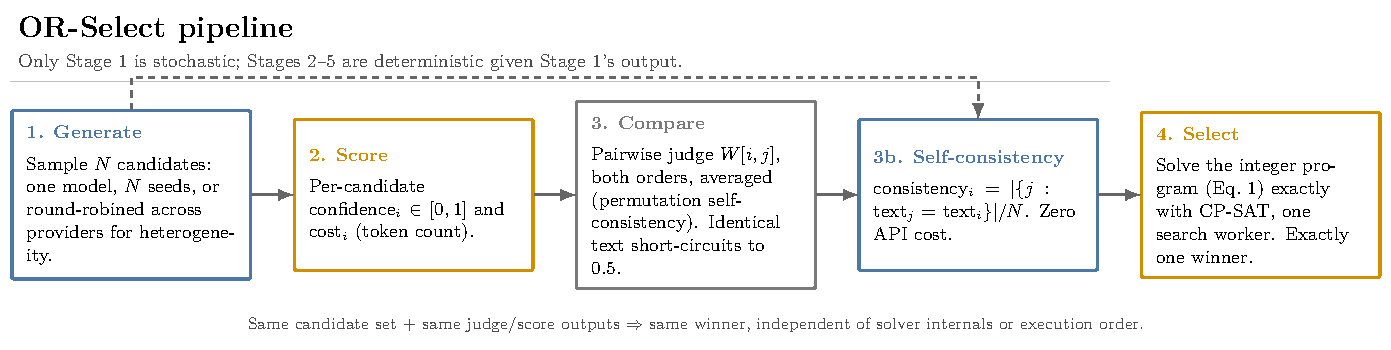
\includegraphics[width=\textwidth]{Figure_1_Pipeline.pdf}
\caption{OR-Select. Generation and judge calls may be stochastic; aggregation
and selection use their stored outputs. Self-consistency requires no API calls.}
\label{fig:pipeline}
\end{figure}

Sample $N$ candidates from one model or a round-robin model pool.
An invalid slot (for example, no extractable answer letter) is retried up
to three times with varied seeds; persistent failures are reported as
ungraded. Confidence $C_i\in[0,1]$ comes from a judge call, cost $c_i$ is
word count, and consistency $K_i=|\{j:\text{text}_j=\text{text}_i\}|/N$
counts exact full-text matches, unlike final-answer voting.

For each unordered pair, average the judge's forward score and the
complement of its reverse score to obtain $W[i,j]\in[0,1]$; set
$W[j,i]=1-W[i,j]$. This symmetrization mitigates order effects but does
not guarantee unbiased judging. Identical texts after trimming skip the
judge and receive $0.5$. At most $N(N-1)$ comparison calls are needed.
The quality aggregate is $Q_i=(N-1)^{-1}\sum_{j\ne i}W[i,j]$.

The two agreement signals serve different purposes. $Q_i$ measures how
strongly the judge prefers candidate $i$ to its competitors; $K_i$ measures
literal repetition of its complete response. Two derivations that end in
the same number can therefore contribute two votes to the self-consistency
baseline while each has $K_i=1/N$ in the composite objective. Confidence
is a separate pointwise judge assessment, not an observed correctness
frequency. Keeping these quantities separate makes it possible to remove
or reweight one without changing the saved comparisons.

\subsection{Formal Model}
\label{sec:formal-model}

Let $x_i$ indicate selection and $v_i$ denote validity. The selector solves

\begin{equation}
\max \sum_i x_i\left(w_1Q_i+w_2C_i+w_4K_i-w_3c_i\right)
\label{eq:selection-obj}
\end{equation}
\begin{align}
\text{s.t.}\quad & \sum_i x_i=1,\qquad x_i\in\{0,1\}, \\
& x_i\le v_i\quad\text{if some candidate is valid}, \\
& x_i=0\quad\text{if }Q_i<\text{min\_quality}\quad\text{(optional)}.
\end{align}

The default $(w_1,w_2,w_4,w_3)=(1,0.2,0.3,0.01)$ was fixed before
ground-truth runs, without tuning. A hundred-word difference therefore
costs one full quality unit. Without additional constraints, this
one-hot program is simply an argmax; integer programming provides a common
implementation for the eligibility constraints. CP-SAT \citep{perron2023ortools}
maximizes scores rounded after multiplication by $10^4$, using one worker.
Reproducibility is conditional on the stored inputs and solver environment;
this does not establish a canonical optimum across solver versions.

All terms are linear once the candidates have been scored. The validity
constraint excludes invalid candidates if at least one valid candidate
exists; an optional minimum-quality threshold excludes candidates below
that threshold. Thus feasibility restrictions and preference weights have
different roles. A low-cost response is not permitted to bypass an active
validity restriction, while an eligible response can win through a
combination of quality, confidence, consistency and cost. Reporting the
component scales is consequently important even when the final
optimization is computationally elementary.

Rows storing confidence and $W$ permit offline weight changes. The default
replay reproduces \AblationFidelityK/\AblationFidelityN{} extracted final
answers; this comparison is at the final-answer level. A worked example is
in the Online Supplement (Table~\ref{S-tab:worked-example}).

\subsection{Exact Kemeny--Young Baseline}
\label{sec:kemeny-exact}

For the ranking reference, let $y_{ij}=1$ mean that $i$ ranks above $j$.
The Kemeny--Young program maximizes agreement with the same matrix:

\begin{equation}
\max \sum_{i \neq j} W[i,j]\, y_{ij}
\label{eq:kemeny-obj}
\end{equation}
\begin{align}
\text{s.t.} \quad & y_{ij} + y_{ji} = 1 \quad \forall\, i \neq j \label{eq:kemeny-antisym}\\
& y_{ij} + y_{jk} + y_{ki} \leq 2 \quad \forall \text{ distinct } i,j,k \label{eq:kemeny-transitivity}\\
& y_{ij} \in \{0,1\}
\end{align}

Antisymmetry and the absence of 3-cycles enforce a linear order.
The implementation uses $\binom{N}{2}$ binary variables, $O(N^3)$
constraints and coefficients $\operatorname{round}(10^4(W[i,j]-W[j,i]))$.
A 200{,}000-conflict budget replaces a wall-clock limit; a non-optimality
flag distinguishes feasible from proven-optimal solutions. All
\KYTopOneN{} stored reference solutions at $N\le6$ are flagged optimal
for this integerized objective, not necessarily for unrounded weights.

The reference removes the composite selector's confidence, consistency and
cost terms and uses all pairwise relations simultaneously. With cyclic
preferences, its top-ranked candidate need not have the largest weighted
win total. This permits an empirical distinction between losing
information through aggregation and receiving unhelpful information from
the judge. We compare returned answers, rather than treating a difference
between rankings as an accuracy error. When two different candidates give
the same extracted answer, they count as the same answer-level decision.

\subsection{Approximation Guarantee}
\label{sec:approx-guarantee}

\begin{proposition}[Weighted-win ranking]
\label{prop:copeland-approx}
Assume nonnegative pair weights with $W[i,j]+W[j,i]=1$.
Ranking by decreasing $Q_i$ approximates minimum weighted disagreement
within a factor of 5. This factor is tight.
\end{proposition}

The constructed matrix satisfies these conditions. This guarantee, from
\citet{coppersmith2006ordering},
covers the \emph{full quality-only ranking}, not top-1 correctness, agreement
with the Kemeny winner, or the composite objective~\eqref{eq:selection-obj}.

\section{When can a judge beat voting? Pairwise-accuracy thresholds}
\label{sec:theory}

\paragraph{Model} Three candidates are independently correct with probability
$p$, all correct candidates share the same final answer, and wrong answers
are pairwise distinct. Plurality voting breaks answer ties uniformly.
Conditional on the correctness labels, the judge's three \emph{binary}
comparisons are independent: a mixed pair favors the correct candidate
with probability $q$, and a same-class pair is a fair coin. Copeland
selects the candidate with most wins, with an independent uniform tie-break.
This quality-only model differs from the empirical selector's averaged
soft scores and composite objective.

\begin{theorem}[Pairwise-accuracy threshold]
\label{thm:threshold}
Under the model above, the accuracy of the Copeland selector minus the accuracy of plurality
voting is
\[
\Delta(p,q)\;=\;p(1-p)\Bigl[(1-p)(2q-1)(q+1)\;-\;p\,(3-2q)(1-q)\Bigr].
\]
Hence, for $p\in(0,1)$ and $q<1$, the judge-based selector is strictly more accurate than voting
if and only if $\frac{p}{1-p}<\frac{(2q-1)(q+1)}{(3-2q)(1-q)}$; at $q=1$ it is always more accurate. In particular, (i) a judge at
chance ($q=\tfrac12$) selects with accuracy exactly $p$ and loses to voting by
$p^{2}(1-p)$; (ii) the unique break-even accuracy $q^{*}(p)$ increases strictly from $\tfrac12$
(as $p\to0$) to $1$ (as $p\to1$).
\end{theorem}

\begin{proof}
Conditional on exactly $k$ correct candidates, write $a_k$ for Copeland's
correct-selection probability. Then $a_0=0$, $a_3=1$.
With one correct candidate, winning both mixed comparisons succeeds;
winning exactly one succeeds only through a three-way tie, giving
$a_1=q^2+\tfrac13q(1-q)$. With two correct candidates, winning both
mixed comparisons succeeds; a split gives a correct selection with
probability $\tfrac12+\tfrac12\cdot\tfrac23=\tfrac56$, hence
$a_2=q^2+\tfrac53q(1-q)$. Plurality's conditional probabilities are
$(0,\tfrac13,1,1)$. Weighting by $\mathrm{Bin}(3,p)$ gives
\[
\Delta=3p(1-p)^2(a_1-\tfrac13)+3p^2(1-p)(a_2-1),
\]
which simplifies to the stated expression. At $q=\tfrac12$ it equals
$-p^2(1-p)$. On $(\tfrac12,1)$ the ratio in the theorem increases
continuously from zero to infinity: its numerator increases and its
positive denominator decreases. Equating it to $p/(1-p)$ establishes
uniqueness, monotonicity and the endpoint limits of $q^*$.
\end{proof}

At $p=0.8$, $q^*=0.803515\ldots$ (Table~\ref{tab:threshold}).
The formula gives both the sign and size of the gain under the model;
\texttt{scripts/judge\_threshold\_theory.py} checks it by exact enumeration.

An explicit expression for the break-even point is
\begin{equation}
q^*(p)=\frac{2(1+2p)}{1+4p+\sqrt{9+8p-16p^2}}.
\label{eq:threshold-root}
\end{equation}
It follows by setting $\Delta=0$ and rationalizing the relevant root of
$2(1-2p)q^2+(1+4p)q-(1+2p)=0$; the expression also covers $p=1/2$.
For $p=0.8$, plurality accuracy is $0.928$. A judge with $q=0.8$ yields
$0.92672$, just below voting, while $q=0.9$ yields $0.96128$, a gain of
$3.328$ percentage points. At $q=1$, the selector finds a correct candidate
whenever one exists, reaching $0.992$. Thus the threshold is not a claim
that judging cannot help: it identifies the reliability at which its
benefit overtakes the information already supplied by answer repetition.

\begin{table}[htbp]
\centering
\caption{Break-even binary judge accuracy $q^{*}$ at which the Copeland selector
ties plurality voting, as a function of the per-candidate accuracy $p$
(Theorem~\ref{thm:threshold}, $N=3$).}
\label{tab:threshold}
\small
\begin{tabular}{rr}
\toprule
$p$ & $q^{*}(p)$ \\
\midrule
\ThresholdRows
\bottomrule
\end{tabular}
\end{table}

\paragraph{Extensions and limits}
The Online Supplement (Section~\ref{S-sec:s-threshold}) enumerates
$N\le7$ and models wrong-answer collisions: each wrong candidate takes a
shared attractor with probability $\rho$, otherwise a distinct answer.
At $p=0.8,\rho=0$, the computed threshold rises from $0.804$ for $N=3$
to $0.945$ for $N=7$; at $\rho=0.5$ it is approximately $0.82$ for
$N=4,\ldots,7$. A monotone-coupling result bounds a pair-dependent
judge using its \emph{minimum and maximum} mixed-pair accuracies, not their
average (Corollary~\ref{S-cor:pairdep}). The supplement also gives a
large-$N$ threshold lower bound and consistency regimes. Neither candidate
independence nor uniform judge accuracy follows from a high aggregate
benchmark score, and asymptotic voting consistency does not exclude
finite-pool improvements by a stronger judge.

The finite-pool computation conditions on the number $k$ of correct
candidates. Let $a_{N,k}(q)$ denote the probability that a uniformly
tie-broken Copeland winner is correct. Enumerating all binary tournament
outcomes gives
\begin{equation}
A_J(N,p,q)=\sum_{k=0}^{N}\binom Nk p^k(1-p)^{N-k}a_{N,k}(q).
\label{eq:judge-general}
\end{equation}
With distinct wrong answers, plurality succeeds whenever $k\ge2$ and
with probability $1/N$ when $k=1$, so
\begin{equation}
A_V(N,p)=1-(1-p)^N-(N-1)p(1-p)^{N-1}.
\label{eq:vote-general}
\end{equation}
The computed break-even point equates these two accuracies. This is
exhaustive enumeration of the finite comparison model, not an estimate
from the benchmark observations; numerical root finding locates the
crossing to the reported precision. The supplement compares it with an
independent Monte Carlo calculation.

Table~\ref{tab:threshold-n} illustrates the effect of wrong-answer
collisions. Shared wrong answers strengthen the competing wrong vote,
whereas with distinct wrong answers two correct candidates suffice for
plurality to succeed. The collision model changes the voting calculation;
its binary judge still uses the stipulated mixed-pair accuracy. Its
parameter $\rho$ describes a common wrong answer, not arbitrary dependence
between candidate correctness events.

\begin{table}[htbp]
\centering
\caption{Finite-pool break-even binary accuracy $q^*(p,N,\rho)$, computed
by exhaustive tournament enumeration. A wrong candidate takes a shared
wrong answer with probability $\rho$, otherwise a distinct wrong answer.}
\label{tab:threshold-n}
\small
\begin{tabular}{rrrrr}
\toprule
 & \multicolumn{2}{c}{$\rho=0$} & \multicolumn{2}{c}{$\rho=0.5$} \\
\cmidrule(lr){2-3}\cmidrule(lr){4-5}
$N$ & $p=0.5$ & $p=0.8$ & $p=0.5$ & $p=0.8$ \\
\midrule
\ThresholdNRows
\ThresholdNSevenRow
\bottomrule
\end{tabular}
\end{table}

The pair-dependent extension uses a coupling rather than substituting an
average accuracy. Hold the correctness labels and comparison random
numbers fixed, and increase one mixed-pair accuracy. The only possible
change gives a correct candidate one additional win and a wrong candidate
one fewer win; the correct fraction of the top-score set cannot decrease.
Applying this change successively bounds selection accuracy between the
uniform-$q_{\min}$ and uniform-$q_{\max}$ cases. This provides a conservative
comparison when such bounds are available, without requiring every mixed
pair to have exactly the same reliability.

\subsection{Problems of differing difficulty}
\label{sec:mixture}

Theorem~\ref{thm:threshold} treats $p$ as common to all problems. In a
benchmark, difficulty varies: many problems are solved by every candidate or
by none, and only intermediate problems separate the rules. Let $p$ be drawn
per problem from a distribution $F$, with candidates and comparisons following
the model given $p$. Write $A(q)=(2q-1)(q+1)$ and $B(q)=(3-2q)(1-q)$, so that the
single-$p$ gap of Theorem~\ref{thm:threshold} is
$A(q)\,p(1-p)^2-B(q)\,p^2(1-p)$.

\begin{theorem}[Effective-odds threshold]
\label{thm:mixture}
Let $m_1=\mathbb{E}_F[p(1-p)^2]>0$ and $m_2=\mathbb{E}_F[p^2(1-p)]$. The accuracy of
Copeland minus that of plurality is $\Delta_F(q)=A(q)\,m_1-B(q)\,m_2$. It is positive
if and only if $A(q)/B(q)>r_F:=m_2/m_1$, so the break-even accuracy $q^*_F\in(\tfrac12,1]$
is the unique root of $A/B=r_F$ and increases with $r_F$.
\end{theorem}

The pooled threshold of Theorem~\ref{thm:threshold} is the special case
$F=\delta_{\bar p}$, where $r_F=\bar p/(1-\bar p)$. Dispersion changes $r_F$, so two
benchmarks with the same mean accuracy can have different break-even
judges; Table~\ref{tab:mixture} gives Beta examples. A problem set needs no
parametric $F$: if problem $i$ has $k_i$ of 3 candidates correct, the
conditional accuracy of Copeland is $a_{k_i}(q)$ (closed forms in the proof of
Theorem~\ref{thm:threshold}) and that of plurality is $0,\tfrac13,1,1$ for $k_i=0,\dots,3$.
Averaging over the observed $k_i$ gives a prediction that uses the
problems' own difficulty (Section~\ref{sec:mixture-results}).

\begin{table}[htbp]
\centering
\caption{Break-even binary accuracy $q^*_F$ when $p\sim\mathrm{Beta}$ with mean $\bar p$
and concentration $\kappa$ (smaller $\kappa$ means more dispersed difficulty);
the last column is the single-$p$ threshold at $\bar p$.}
\label{tab:mixture}
\small
\begin{tabular}{rrrrrr}
\toprule
$\bar p$ & $\kappa=1$ & $\kappa=2$ & $\kappa=5$ & $\kappa=20$ & $p\equiv\bar p$ \\
\midrule
\MixtureThresholdRows
\bottomrule
\end{tabular}
\end{table}

\subsection{Vote first, judge only on ties}
\label{sec:hybrid}

The model says more than a threshold. Because correct candidates share an
answer and wrong answers are distinct, any repeated answer is certainly
correct. A judge can only help when all $N$ answers differ. Rule~H returns a
most-voted answer and, if several answers tie, runs binary Copeland on the
comparisons among the tied candidates only.

\begin{theorem}[Vote-first fusion is optimal]
\label{thm:hybrid}
Under the model, for any $N\ge 2$ and $q\ge\tfrac12$, Rule~H attains the maximum
accuracy among all rules that observe the answer partition and the
comparison outcomes, namely
$P(k\ge2)+N\,p(1-p)^{N-1}\,a^{(N)}(q)$, where $a^{(N)}(q)\ge 1/N$ is the probability
that Copeland selects the lone correct candidate among $N$ distinct answers. Hence
Rule~H is at least as accurate as plurality and as Copeland for every $p$
and $q\ge\tfrac12$: it has no break-even threshold.
\end{theorem}

The proof (Appendix) is a Bayes argument: when all answers differ, the
posterior of a candidate being the only correct one is proportional to
$q^{w}(1-q)^{N-1-w}$, increasing in its number of wins $w$. Exhaustive
enumeration for $N\le4$ in exact rational arithmetic and for $N=5,6$ in floating
point confirms optimality and dominance. For example, at $N=6$, $p=0.3$ and
$q=0.8$ the accuracies of plurality, Copeland and Rule~H are $63.0\%$, $70.7\%$
and $77.1\%$ (Table~\ref{tab:hybrid-theory}). The result is a design principle
for fusion: spend judge calls only where votes are uninformative. It is also a
cost statement. Rule~H compares only when all $N$ answers differ, which in the model
happens with probability $P(k\le1)=(1-p)^N+Np(1-p)^{N-1}$ and then needs $\binom N2$
comparisons, so its expected number of comparisons is $\binom N2\,P(k\le1)$ against
$\binom N2$ for Copeland on every problem; at $N=3$ and $p=0.6$ this is $0.35$ of the
comparisons. The result is proved
only for distinct wrong answers; when wrong answers collide, a wrong repeated
answer can outvote a lone correct one, Rule~H inherits that failure, and a
Copeland-based rule can recover it (Table~\ref{tab:threshold-n}).

\begin{table}[htbp]
\centering
\caption{Model accuracy (\%) of plurality, Copeland and Rule~H (exact enumeration).}
\label{tab:hybrid-theory}
\small
\begin{tabular}{rrrrrr}
\toprule
$N$ & $p$ & $q$ & Plurality & Copeland & Rule~H \\
\midrule
\HybridTheoryRows
\bottomrule
\end{tabular}
\end{table}

\section{Experimental Protocol}
\label{sec:experiments}

\subsection{Setup}
\label{sec:setup}

The fixed judge is NVIDIA Nemotron-3.5-Lightning on OpenRouter
(\texttt{\seqsplit{nvidia/nemotron-3.5-lightning:free}}), with reasoning
disabled and a 256-token cap; truncated judge replies raise errors.
Homogeneous pools contain $N=3$ Nemotron draws with distinct seeds.
Heterogeneous pools contain $N=6$ draws, initially two each from Nemotron,
Poolside Laguna-S~2.1 and Cohere North-Mini-Code. After Laguna's withdrawal,
Xing4.0-29B filled its slots (\SelectionXingchenCands{} candidates);
one early GPQA problem retains two LFM-2.5 candidates. This pool drift is
reported, not treated as a fixed three-model experiment.

Generation uses a 32{,}768-token cap and varied-seed retries. A flagged
second pass retries ungraded problems at 65{,}536 tokens, subject to model
ceilings. Tables~\ref{S-tab:coverage}--\ref{S-tab:extended} report coverage,
pool composition and accuracy with and without these rescued problems.

The main references are self-consistency (plurality over extracted final
answers, candidate-order ties), the \emph{first sampled candidate} (not
temperature-zero greedy decoding), and the Kemeny--Young top-ranked answer
on the same matrix. Further offline selectors are listed in
Section~\ref{sec:baselines}. Trained verifiers and universal
self-consistency were not evaluated.

\paragraph{Judge calibration}
\label{sec:rewardbench-setup}

RewardBench \citep{rewardbench2025} uses the same forward/backward judging
path: its combined score must favor the human-preferred answer. The
pre-registered sample takes the first seven rows of each of 23 subsets
($n=161$), not a random sample. Overall accuracy averages category means;
the supplement also reports a micro-average and its Wilson interval.

\subsection{Evaluation tracks}
\label{sec:tracks}

Six homogeneous tracks comprise \TotalProblems{} distinct problems:
B, 40 GSM8K test items \citep{cobbe2021gsm8k}; C, all 134 Level-5 items
of MATH-500 \citep{hendrycks2021math,lightman2023letsverify}; D, 30 AIME
2026 problems \citep{matharena2025aime}; E, all 198 GPQA Diamond items
\citep{rein2024gpqa}; F, 30 AIME 2025 problems; and G, 100 MMLU-Pro test
items \citep{wang2024mmlupro}. B--E are repeated with heterogeneous pools
on the same 402 problems, not additional independent benchmark items.
MMLU-Pro samples five consecutive items at each of 20 evenly spaced
offsets, covering 12 of 14 subjects. AIME 2025 may be contaminated because
it predates the generator; it is a robustness check.

GSM8K uses the last number; MATH uses normalized exact match of the last
\texttt{\textbackslash boxed\{\}} answer; AIME uses the extracted integer;
GPQA and MMLU-Pro use exact letters. String-based mathematics grading can
reject equivalent expressions. The three-query open-ended pilot has no
ground truth and is supplementary only (Section~\ref{S-sec:pilot}).

\subsection{Metrics}
\label{sec:metrics}

We report graded/benchmark-total coverage and exact two-sided McNemar tests
on paired discordant problems \citep{fagerland2013mcnemar}; pooled tests sum
discordances within each generation condition. The test form was
pre-registered, but the added tracks and six-track homogeneous pooling were
not; pooled findings, per-track comparisons and ablations are exploratory,
without multiplicity correction. A non-significant test is not equivalence.

The \emph{floor} is mean candidate accuracy (uniform random selection),
not a performance lower bound; the \emph{oracle} is the proportion with
at least one correct candidate. Recovery is
$(\mathrm{acc}-\mathrm{floor})/(\mathrm{oracle}-\mathrm{floor})$
\citep[cf.][]{landesberg2026bestofn}, reported only when headroom is positive.
Negative recovery means worse than a random pick.

\section{Results}
\label{sec:results}

\subsection{Judge validation: RewardBench}
\label{sec:rewardbench-results}

The fixed judge scores \RBOverallAcc\% overall, reaching
\RBReasoningAcc\% on reasoning pairs (\RBReasoningCorrect/\RBReasoningRows).
Rotating judges yields \RBXOverallAcc\%; this exploratory result informed
retaining one fixed judge. Table~\ref{tab:rewardbench} separates the
categories. This calibration evaluates agreement with human-preferred
responses; it is not the binary correct-versus-wrong parameter of the
threshold model. Micro-averaging, length diagnostics and configuration
history appear in Section~\ref{S-sec:judge-diagnostics} of the Online
Supplement.

\begin{table}[htbp]
\centering
\caption{Fixed-judge RewardBench accuracy by category ($n=\RBN$).
The overall score is the mean of category accuracies.}
\label{tab:rewardbench}
\begin{tabularx}{\textwidth}{Xrr}
\toprule
Category & Rows & Accuracy \\
\midrule
Reasoning (math-prm and six \texttt{hep-*} code subsets) & \RBReasoningRows & \RBReasoningAcc\% \\
Chat & \RBChatRows & \RBChatAcc\% \\
Chat Hard (adversarial LLMBar subsets) & \RBChatHardRows & \RBChatHardAcc\% \\
Safety & \RBSafetyRows & \RBSafetyAcc\% \\
\bottomrule
\end{tabularx}
\end{table}

\subsection{Accuracy against the baselines}
\label{sec:accuracy-results}

Tables~\ref{tab:tracks}--\ref{tab:paired} report accuracy and paired
discordances. Across \HomogPooledN{} homogeneous problems, OR-Select
alone is correct on \HomogPooledB{} and self-consistency alone on
\HomogPooledC{} (\HomogPooledP): a difference of $-0.56$ percentage
points, without a detected advantage. Across \HeteroPooledN{} heterogeneous
problems the counts are \HeteroPooledB{} versus \HeteroPooledC{}
(\HeteroPooledP), a $-5.47$-point difference. This loss comes from GSM8K,
MATH and AIME 2026. Heterogeneous GPQA instead favors OR-Select numerically
(10 versus \SCwinsGPQAx{} discordances, $p=0.454$), so the pooled result
is not uniform across tasks.

\begin{table}[htbp]
\centering
\caption{Accuracy (\%) on graded problems, by track and selector. `--': no
Kemeny--Young comparator (GSM8K). Bold: best of the three practical
selectors when they differ. Primed rows: heterogeneous generation.}
\label{tab:tracks}
\small\setlength{\tabcolsep}{4pt}
\resizebox{\textwidth}{!}{%
\begin{tabular}{lrrrrr}
\toprule
Track & Graded/Total & First sample & Self-cons.\ & OR-Select & Kemeny--Young \\
\midrule
\TracksTableRows
\bottomrule
\end{tabular}}
\end{table}

\begin{table}[htbp]
\centering
\caption{Paired comparison of OR-Select with each reference selector. Cells
give (problems where OR-Select is right and the reference wrong)/(the
reverse) and the exact two-sided McNemar $p$-value.}
\label{tab:paired}
\small\setlength{\tabcolsep}{3pt}
\resizebox{\textwidth}{!}{%
\begin{tabular}{lrrrrrr}
\toprule
Track & vs.\ SC & $p$ & vs.\ first sample & $p$ & vs.\ Kemeny--Young & $p$ \\
\midrule
\PairedTableRows
\bottomrule
\end{tabular}}
\end{table}

\subsection{Headroom and recovery}
\label{sec:recovery}

Table~\ref{tab:recovery} distinguishes saturation from failed selection.
Homogeneous GSM8K has no headroom; homogeneous GPQA has roughly ten
percentage points, of which both selectors recover 16\%.
OR-Select falls below the random-pick floor on heterogeneous MATH and
AIME 2026, whereas its numerical recovery advantage on heterogeneous GPQA
is not statistically significant (Table~\ref{tab:paired}).

\begin{table}[htbp]
\centering
\caption{Headroom and recovery on graded problems. Floor: mean candidate
accuracy. Oracle: some candidate correct. Recovery (\%):
$(\text{acc}-\text{floor})/(\text{oracle}-\text{floor})$; negative means
below a random pick.}
\label{tab:recovery}
\small\setlength{\tabcolsep}{4pt}
\resizebox{\textwidth}{!}{%
\begin{tabular}{lrrrrrrr}
\toprule
Track & Graded & Floor & SC & OR & Oracle & Rec.\ SC & Rec.\ OR \\
\midrule
\RecoveryTableRows
\bottomrule
\end{tabular}}
\end{table}

\subsection{Objective and selection diagnostics}
\label{sec:selection-bias}
\label{sec:cost-diagnosis}
\label{sec:ablations}

On replayable problems, the within-pool cost-term spread has median
\CostSpreadMed{}, versus \QualitySpreadMed{} for quality, and exceeds
the quality spread in \CostDominatesK/\CostDominatesN{} cases. This
exposes a scale mismatch, not a proof that cost determines every winner:
confidence, consistency, eligibility and score gaps also matter.

Table~\ref{tab:ablation} compares the default, no-cost, quality-only and
plurality-plus-quality variants on identical replayable subsets. In
heterogeneous pools, removing cost yields \AblHetNoCostAcc\% accuracy and
quality-only selection \AblHetQOnlyAcc\%, against voting's
\AblHetSCAcc\% ($n=\AblHetN$; exact $p$ \AblHetNoCostP{} and
\AblHetQOnlyP{}, respectively). Thus the cost term is not the only
limitation. These post-hoc results do not prove that the judge contains
no useful correctness information.

OR-Select picks Cohere candidates in \PickShareCohere\% of heterogeneous
problems, although their overall accuracy (\CandAccCohere\%) is similar to
Nemotron's (\CandAccNemotron\%). This is a property of the \emph{composite
selector}, not an isolated judge preference; length and other terms are
confounded (Table~\ref{S-tab:selection}).

\begin{table}[htbp]
\centering
\caption{Offline replay of the selection step on stored judge outputs
(accuracy \%, problems whose judge outputs were stored). SC: stored
self-consistency result on the same problems.}
\label{tab:ablation}
\small\setlength{\tabcolsep}{4pt}
\resizebox{\textwidth}{!}{%
\begin{tabular}{lrrrrrr}
\toprule
Track & Replayable & SC & Default & No cost & Quality only & SC+quality \\
\midrule
\AblationTableRows
\bottomrule
\end{tabular}}
\end{table}

\paragraph{Additional selectors}
\label{sec:baselines}

Shortest/longest, token-Jaccard minimum-Bayes-risk, pointwise confidence,
confidence-weighted voting, a knockout tournament and Bradley--Terry
selection establish no significant improvement over plurality in the
exploratory comparisons (Table~\ref{S-tab:baselines}). Minimum-Bayes-risk
is numerically ahead in some pooled comparisons, without a significant advantage.

\paragraph{Soft-score diagnostics}
\label{sec:threshold-results}

The mean stored weight assigned to the correct candidate on mixed pairs
is $0.49$--$0.56$ on tracks with at least 70 such pairs. These are
\emph{soft-score means}, not frequencies of correct binary decisions.
They cannot be substituted for $q$ in Theorem~\ref{thm:threshold}; neither
can an average establish the pairwise bounds of Corollary~\ref{S-cor:pairdep}.
Table~\ref{S-tab:threshold-emp-gen} retains these descriptive measurements
and model sensitivity calculations, with their sampling limitations.

\subsection{Difficulty-aware prediction}
\label{sec:mixture-results}

On the homogeneous problems with stored judge outputs and at least ten mixed
pairs ($n=\MixPooledN$, AIME 2025 and MMLU-Pro; GSM8K has no stored judgments and
MATH Level 5 and AIME 2026 have too few mixed pairs), the binary mixed-pair
accuracy is $\MixPooledQ\%$. Using each problem's own number of correct
candidates $k_i$ and this $q$, the model predicts binary-Copeland accuracy
$\MixPooledPredCop\%$; the observed value is $\MixPooledObsCop\%$ (bootstrap
interval for observed minus predicted, re-estimating $q$ in each resample:
$[\MixPooledErrLo,\MixPooledErrHi]$ points). A pooled-$p$ prediction under the
single-$p$ binomial model gives $\MixPooledNaiveCop\%$. The two agree on Copeland but not on plurality: observed plurality
accuracy is $\MixPooledObsVote\%$, the own-$k$ model gives $\MixPooledPredVote\%$ and the pooled-$p$ model
$\MixPooledNaiveVote\%$, because the binomial model puts too little mass on problems solved by
none or one candidate. The resulting gap prediction (Copeland minus plurality, in points)
is $\MixPooledGapPred$ with own $k_i$ against $\MixPooledGapNaive$ pooled, for an observed
$\MixPooledGapObs$ (Table~\ref{tab:mixture-emp}). The sample is small and $q$ is estimated on the
same rows, so this is a plug-in consistency check, not out-of-sample validation;
MMLU-Pro's binary $q$ lies below one half on 28 mixed pairs.

\begin{table}[htbp]
\centering
\caption{Observed and predicted binary-Copeland accuracy (\%) and the Copeland-minus-plurality
gap (points). Pred.\ ($k_i$) uses each problem's own number of correct candidates;
Pred.\ ($\bar p$) uses the single-$p$ binomial model at the pooled accuracy.}
\label{tab:mixture-emp}
\scriptsize
\setlength{\tabcolsep}{3pt}
\begin{tabular}{lrrrrrrrrr}
\toprule
 & & & & \multicolumn{3}{c}{Copeland accuracy} & \multicolumn{3}{c}{Gap} \\
\cmidrule(lr){5-7}\cmidrule(lr){8-10}
Track & $n$ & $\hat p$ & $\hat q$ & Obs. & $k_i$ & $\bar p$ & Obs. & $k_i$ & $\bar p$ \\
\midrule
\MixtureEmpiricalRows
\bottomrule
\end{tabular}
\end{table}

\subsection{Vote-first fusion on stored runs}
\label{sec:hybrid-results}

Rule~H is computed offline on every graded problem with stored judge outputs
($\HybHomN$ homogeneous and $\HybHetN$ heterogeneous problems; Table~\ref{tab:hybrid-audit}).
Exact vote ties are rare: $\HybHomTies$ and $\HybHetTies$ problems, of which only
$\HybHomOpp$ and $\HybHetOpp$ contain a correct candidate. Rule~H therefore tracks voting:
$\HybHetHyb\%$ against $\HybHetSC\%$ in heterogeneous pools ($\HybHetBSC$ versus $\HybHetCSC$ discordant
problems, $p=\HybHetPSC$) and $\HybHomHyb\%$ against $\HybHomSC\%$ in homogeneous pools
($\HybHomBSC$ versus $\HybHomCSC$, $p=\HybHomPSC$). Against Copeland alone it is better in heterogeneous
pools ($\HybHetBCop$ versus $\HybHetCCop$ discordant problems, $p=\HybHetPCop$) and indistinguishable
in homogeneous pools ($\HybHomBCop$ versus $\HybHomCCop$). Using the judge only on ties thus removes
the heterogeneous-pool penalty of judging everywhere, but with the tested judge it adds no
detectable accuracy over voting, as expected when its binary accuracy is near chance. Its practical
benefit is cost: because the judge is consulted only on ties, Rule~H needs $\HybHomCallShare\%$
(homogeneous) and $\HybHetCallShare\%$ (heterogeneous) of the pairwise comparisons that Copeland on
every problem requires, avoiding $\HybHomCallSaved\%$ and $\HybHetCallSaved\%$ of judge comparisons at
voting-level accuracy. The stored
voting baseline breaks ties by candidate order, and the judged subset is not a random sample;
GPQA Diamond is not part of this audit because its stored outputs are not in the public archive.

\begin{table}[htbp]
\centering
\caption{Rule~H on stored runs. Ties: problems where several answers tie for most votes; Opp.:
ties containing a correct candidate. Accuracy in \%. Discordant counts are problems won by
Rule~H and lost by the comparator, with the exact two-sided McNemar $p$ in parentheses.}
\label{tab:hybrid-audit}
\scriptsize
\setlength{\tabcolsep}{3pt}
\begin{tabular}{lrrrrrrr}
\toprule
Track & $n$ & Ties/Opp. & Vote & Copeland & Rule H & H vs.\ vote & H vs.\ Copeland \\
\midrule
\HybridAuditRows
\bottomrule
\end{tabular}
\end{table}

\subsection{Ranking reference and coverage}
\label{sec:kemeny-results}

OR-Select and the integerized Kemeny--Young reference return different
final answers on \KYTopOneDiffers/\KYTopOneN{} problems. OR-Select alone
is correct on \KYORwins{} and Kemeny--Young alone on \KYKYwins{}
(Table~\ref{tab:paired}); the exact ranking reference shows no detected
accuracy advantage. Ranking optimality does not guarantee correctness.

\paragraph{Coverage}
\label{sec:coverage}

Every problem is ultimately graded (Table~\ref{S-tab:coverage}). Including
the higher-cap rescued problems lowers selector accuracy by 0.3--15 points
depending on track, without reversing the direction of the comparisons
(Table~\ref{S-tab:extended}). These results describe the retry-conditioned
generation protocol, not unrestricted independent draws.

\section{Design guidelines for system builders}
\label{sec:guidelines}

The results translate into five guidelines for the answer-selection component of a
language-model system whose final answers can be extracted and compared.
\begin{enumerate}
\item \textbf{Vote first.} Extract each candidate's final answer and return the plurality
answer when it is unique. In the model, this loses nothing against voting and
never needs a judge-accuracy threshold (Theorem~\ref{thm:hybrid}); on the stored
runs no accuracy difference against self-consistency was detected.
\item \textbf{Call the judge only on ties.} Compare only the tied candidates. On the stored runs this
needed \HybHomCallShare\% (homogeneous) and \HybHetCallShare\% (heterogeneous) of the
comparisons that judging every problem requires, and it removed the heterogeneous-pool
loss of judging everywhere (Section~\ref{sec:hybrid-results}).
\item \textbf{Replace voting by judging everywhere only above a measured break-even.}
Estimate the judge's binary accuracy on mixed pairs from a labeled sample, then compare it
with the break-even computed from the observed distribution of correct candidates per problem
(Theorem~\ref{thm:mixture}); pooled accuracy misstates it, and a judge near chance never qualifies.
\item \textbf{Audit on frozen pools.} Store the candidate pool and the judge outputs per problem and
compare selectors on the same problems with paired exact tests on discordant problems. Report
how many problems have ties and how many ties contain a correct candidate, because that
bounds what a tie-breaking judge can add.
\item \textbf{Control judge biases before trusting a judge.} Average both presentation orders, and test
style effects, which one systematic comparison finds larger than position effects
\citep{soumik2026judging} and which this study did not control (Section~\ref{sec:future}).
\end{enumerate}
These guidelines hold under the stated assumptions: answers that can be extracted and compared, and
the tested judge and configuration. They do not show that stronger judges cannot help.

\section{Discussion}

\paragraph{Interpretation}
The audit supports evaluating the entire decision rule on fixed candidate
pools: a ranking objective can fit judge preferences without improving
correctness, and an unnormalized cost term can overshadow a bounded quality
score. Stored outputs make these distinctions inspectable without new API
calls. The theory separately quantifies the trade-off for independent binary
comparisons. Connecting it to soft-score selection requires assumptions
about score distributions and dependence, not merely a mean score.

\paragraph{Scope}
\label{sec:future}

Only one free-tier fixed judge is evaluated in the main audit. Stronger
judges, trained verifiers and other selection architectures may perform
differently. Forward--reverse averaging addresses position bias; style bias,
reported to be larger in other judge benchmarks \citep{soumik2026judging},
is not controlled, and a debiasing comparison on this pool is left open. Small discordant counts limit precision; the replay subset is
not randomly sampled, and mixed-pair measurements are sparse on several
tracks. Candidate-order voting ties can favor particular generators in the
round-robin pool. The reported results describe the generation, extraction
and retry protocols of Section~\ref{sec:experiments}. The theory assumes
independent candidate correctness and
conditionally independent comparisons; the wrong-answer collision model
does not model general correlated errors.

\section{Conclusion}

An exact finite-$N$ calculation specifies when binary Copeland selection
beats plurality under a stylized model; with varying difficulty the
break-even accuracy is set by an effective-odds ratio rather than pooled
accuracy, and a vote-first rule that judges only on ties is optimal in the model
and has no break-even threshold. A separate six-benchmark audit
finds no detected homogeneous-pool advantage for the tested free-tier judge
and a pooled heterogeneous-pool loss; on stored runs, vote-first selection
removes that loss but, because exact ties are rare and the judge is near
chance, adds no detectable accuracy over voting. The exact Kemeny reference and
offline ablations distinguish ranking fit, objective design and answer
accuracy. Together, the finite-pool calculation and stored-output audit
separate the reliability needed by a specified selection rule from the
performance observed for a particular judge configuration.

\section*{Data availability statement}
The code, tables, pre-registration documents and stored run files that support the findings are archived in a
public repository. To preserve anonymity during double-blind review, the persistent identifier is given in the
submission form and an anonymized copy is provided with the submission; the identifier will be cited in the
accepted version. The archive excludes GPQA records containing password-gated question text, which cannot be
redistributed; access to that benchmark follows its distribution conditions. The analysis scripts regenerate all
tables from the stored runs and include the GPQA generation workflow.

\section*{Declaration of competing interest}
The author declares no known competing financial interests or personal relationships
that could have appeared to influence the work reported in this paper.

\section*{Funding}
This research did not receive any specific grant from funding agencies in the public,
commercial, or not-for-profit sectors.

\section*{Declaration of generative AI and AI-assisted technologies in the manuscript preparation process}
During preparation the author used Claude (Anthropic; Claude Code with
Claude Sonnet 5.5) for analysis code, drafting, bibliographic checks and
derivation and numerical verification of the theoretical results, and
OpenCode (GPT-6.1 Sol) for critical review and editorial compression.
The models served through OpenRouter are experimental subjects, not writing tools.
After using these tools the author reviewed and edited the content as needed and takes
full responsibility for the content of the publication.


\bibliographystyle{chicago}
\bibliography{refs}

\end{document}
